\documentclass[fontsize=5pt]{scrartcl}

%
% Original Page by LinuxMercedes
%

\usepackage[
        nohead,
        nofoot,
        left=0.55in,
        right=0.55in,
        top=0.55in,
        bottom=0.55in,
]{geometry}

\usepackage{amsmath,scalefnt}

\usepackage{graphicx}

\renewcommand*{\arraystretch}{.5}

\usepackage{multicol}
\setlength{\columnsep}{5pt}

\usepackage{helvet}
\renewcommand{\familydefault}{\sfdefault}

\pagenumbering{gobble}

\usepackage{enumitem}
\setlist[itemize]{itemsep=-2pt, itemindent=0pt, leftmargin=*}
\setlist[enumerate]{itemsep=-2pt, itemindent=0pt, leftmargin=*}

\usepackage[compact]{titlesec}
\titlespacing{\section}{-1pt}{-1pt}{-1pt}
\titlespacing{\subsection}{-1pt}{-1pt}{-1pt}

\usepackage{listings}

%Y hoy yo reza que no empleo ni alma pobre encontrará esta magica negra.
%This is a custom 'tight' matrix for this cheatsheet. It's ugly.
\newenvironment{tmatrix}%
{ 
  %\scalefont{.5}
  %\setlength{\tabcolsep}{5pt}
  $\left[\hspace{-3.5pt}\begin{array}{c@{\hspace{1pt}}c@{\hspace{1pt}}c@{\hspace{1pt}}|@{\hspace{0pt}}c}
}%
{
   \end{array}\hspace{-3.5pt}\right]$
}

\newenvironment{tmatrix3}%
{ 
  %\scalefont{.5}
  %\setlength{\tabcolsep}{5pt}
  $\left[\hspace{-3.5pt}\begin{array}{c@{\hspace{1pt}}@{\hspace{1pt}}c@{\hspace{1pt}}c@{\hspace{3pt}}}
}%
{
   \end{array}\hspace{-3.5pt}\right]$
}

\newenvironment{tmatrix1}%
{ 
  $\left[\hspace{-3.5pt}\begin{array}{c@{\hspace{3pt}}}
}%
{
   \end{array}\hspace{-3.5pt}\right]$
}


%was 3 3 3 3
\DeclareMathSizes{3pt}{3pt}{3pt}{3pt}

\begin{document}

\begin{multicols}{3}
  \section{Definitions}
    \begin{itemize}
      \item \textbf{Operating Systems}: exploit hardware resources (many processors), provide a set of services to users, manage secondary memory and I/O, %
          and provide networking/comm. support. Elements of an OS:
      \begin{itemize}
        \item Processor
        \item Main Memory (real/primary)
        \item I/O Modules: secondary memory devices, comms equipment, terminals
        \item System bus: communication among processors, memory, and I/O modules
       \end{itemize}
       \item \textbf{Interrupts}: interrupts the normal sequence of execution. Improve processing efficiency and lets the processor not wait on things.
       \item \textbf{ISR}: Interrupt service routine, handles interrupts. Whenever  there is an interrupt, control is transferred to this program.  %
                       It determines the nature of the interrupt and performs the necessary actions to handle it.

    \end{itemize}
     \subsection{Processing}
      \begin{itemize}       
       \item \textbf{Multithreading}: Executing an application using parts of it, which were divided into threads. 
       \item \textbf{Thread}: Dispatchable unit of work, has its own data area and processor context, execute sequentially.
       \item \textbf{Process}: A collection of one or more threads and resources.
       \item \textbf{SMP}: Symmetrix MultiProcessing, multiple, connected, homogenus processors using shared memory.
                           Threads can be scheduled across all processors. Also refers to the hardware model it runs on, with
                           many processors.
        \item \textbf{Starvation}: A process is postponed indefinitely and does not wake. Usually due to resource allocation quirks (starving!).
        \item \textbf{Mutual Exclusion}: aka mutex; only one process may use a resource at a time.
        \item \textbf{Hold \& Wait}: A process holds some resource while waiting for / requesting another. You can either force a process to request all resources ahead of time,
                                    or force it to release all other resources first.
        \item \textbf{Preemption}: OS forces a process to release its resources. 
        \item \textbf{Circular Wait}: A process waits on another process's resources to free up while that process waits on the first one.
                                      Can be prevented with resource request strategies or by having resources ordered with processes waiting for them in order.
      \end{itemize}
      \subsection{Unix}
      \begin{itemize}
        \item \textbf{Unix Concurrency Mechanisms}:
        \begin{itemize}
          \item Shared memory   Signals
          \item Pipes           Messages
          \item Threads         Semaphores
        \end{itemize}
        \item \textbf{Unix Thread Synchronization Primatives}: Mutual exclusion (mutex) locks:
        \begin{itemize}
          \item pthread\_mutex\_lock( )
          \item pthread\_mutex\_trylock( )
          \item pthread\_mutex\_unlock( )
        \end{itemize}
        \item \textbf{Unix Thread Sync. condition variables}: pthread\_cond\_wait( ); pthread\_cond\_signal( );
        \item \textbf{Unix Fork}: child process is spawned with separate data space than parent process, but shares code space.
        \item \textbf{Unix pthread}: thread shares data space, code space, and os resources (file descriptor table), but the have a unique thread ID, 
                                      register state, stack, priority, and PC.
     \end{itemize}    

  \section{Diagrams}
    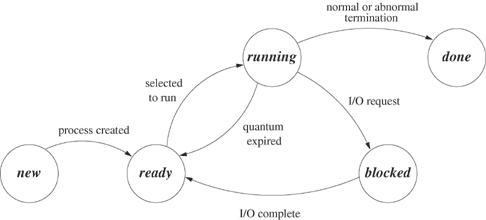
\includegraphics[scale=0.25]{process_state.png} \\
    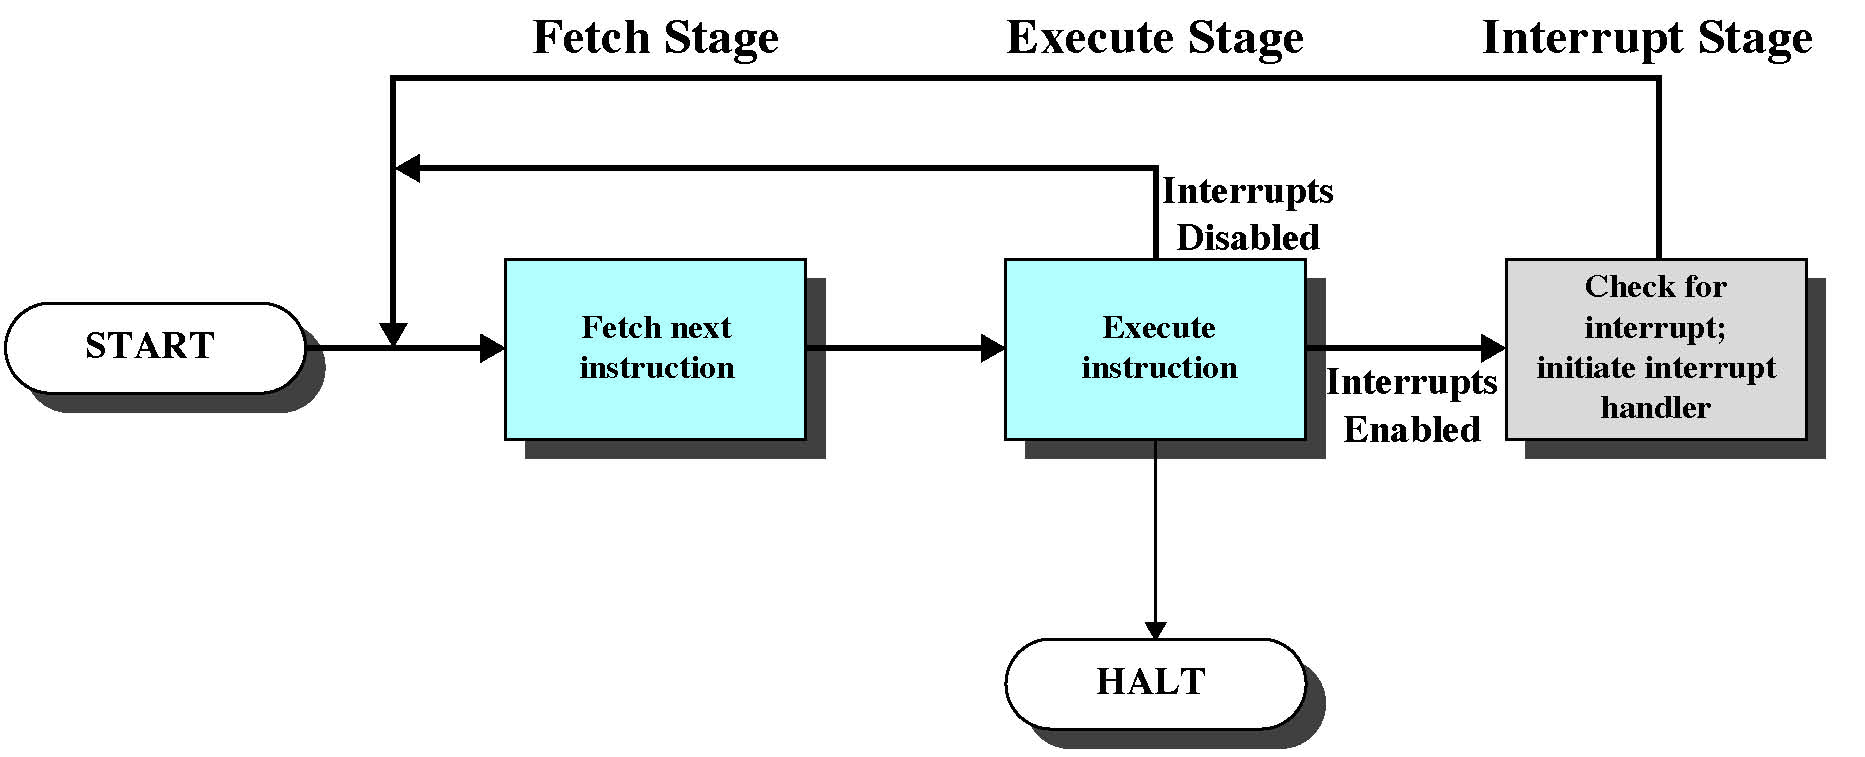
\includegraphics[scale=0.25]{interrupt_cycle.png} \\
    
   \section{Interrupts}
      \begin{itemize}
        \item \textbf{Interrupt Types}: Program interrupts (arithmetic overflow, division by zero, execute illegal instruction), timer, I/O interrupt, HW failure.
      \end{itemize}
    \section{Unix}
      \begin{itemize}
       \item Processor States:
        \begin{itemize}
         \item User Running: executing in user mode.
         \item Kernel Running: executing in kernel mode.
         \item Ready to run, in memory: Ready to run as soon as the kernel schedules it.
         \item Asleep in memory: Unable to execute until an event occurs; process is in main memory, blocked state.
         \item Ready to run, swapped: Ready to run but moved off main memory.
         \item Sleeping, swapped: awaiting an event but moved off main memory.
         \item Preempted: process is returning from kernel to user mode, but the kernel preempts it and does a process switch
               to schedule another process. Very similar/same as ready to run, in memory.
         \item Created: newly created and ready to run.
         \item Zombie: no longer exists and left a record for its parent to clean up.
        \end{itemize}
        \item Unix Modes: user mode, less privileged, usually user programs. System/supervisor/kernel: privileged.
        \item Including signal.h provides:
        \begin{itemize}
          \item Raising with kill(pid, signal); ie kill(1,SIGINT);
          \item Ignoring with signal(num/id, SIG\_IGN);
          \item Handling with signal(num/id, handlerfunc);
        \end{itemize}
        \item Common signals:
        \begin{itemize}
          \item SIGHUP, hangup
          \item SIGINT, Interrupt (ctrl+c)
          \item SIGQUIT, quit (ctrl+\textbackslash)
          \item SIGKILL, kill process
          \item SIGTERM, terminate software
          \item SIGCHLD, child terminated
        \end{itemize}

      \end{itemize}
      
     \section{Threads}
      \begin{itemize}
       \item Many approaches: 
       \begin{itemize}
        \item Single Thread (DOS). One process, one thread.
        \item Multithreaded: Java ``green'' threads, one process many threads.
        \item Unix variants: many processes one thread each.
        \item Windows/Solaris/Unix: Many processes, many threads each.
       \end{itemize}
       \item Threads have their own execution state (running/ready), state is saved when not running, execution stacks, 
             some of their own storage for variables, and access to all memory and resources of its process.
       \item Way cheaper to make and destroy than a new process due to shared memory.
       \item Switching to a thread is cheaper.
      \end{itemize}
      
      \section{Concurrency}
        \begin{itemize}
          \item Mutual Exclusion: Only one process can be in a critical section at a time. Without this, results aren't consistent.
          \item Critical Section: CS. Used a lot to encapsulate important parts of code. It must be ran without interruption or waiting.
          \item Concurrency can be achieved in any of the following ways:
          \begin{itemize}
            \item Disabling interrupts: this guarantees mutual exclusion but is exploitable for user processes. Can be disabled forever.
            \item Lock variables: Processes must have a lock to run or modify variables (GIT). Sleep in process while locked
                  get(lock), run our code, and release(lock).
            \item Semaphores, almost universally using Dijkstra's Semaphore.
          \end{itemize}

       \end{itemize}
       \subsection{Semaphores}
         A \textit{nonnegative} number variable, s can only be changed or tested by two atomic functions:
         \begin{itemize}
          \item $P(s)$: [ while($s<=0$) \{wait\}; s = s-1; ]
          \item $V(s)$: [ s = s + 1; ]
         \end{itemize}
         Semaphores are:
         \begin{itemize}
          \item Conceptualized and have no specific purpose in mind. However, for us, P is get and
                V release.
          \item P is also wait( ), get( ), and pthread\_mutex\_lock( ).
          \item V is also release( ), signal( ), and pthread\_mutex\_unlock( ).
          \item Semaphore locks will add items to a queue as they wait for the lock to release. See Semaphore example.
          \item Starvation and Deadlocks do not happen in Semaphore locks when used properly.
          \item However if two locks in a semaphore are waiting on each other, this deadlocks.
        \end{itemize}
        

       \subsection{Deadlock}
         \begin{itemize}
          \item \textbf{Deadlocks}: One process is waiting on another to finish, round and round. Nothing is processed. This implies starvation but not vice-versa.
          \item Deadlocks will not occur where: $r>(m-1)*p$ (r=\# of resources, m=max resource per process, p=\# of processes)
          \item \textbf{Deadlock Prevention}: See definitions. This can be prevented if any of the following are false:
          \begin{itemize}
            \item No Mutual Exclusion
            \item No (Hold \& Wait)
            \item Preemption allowed
            \item No (Circular Wait)
          \end{itemize}
           \item \textbf{Deadlock Avoidance}: Uses a model with a system of states and a strategy that will guarantee a deadlock state won't happen.
           \begin{itemize}
             \item Can choose a strategy with a system of states to avoid a deadlock state.
             \item Requires extra information (max claim for each process).
             \item Resource manager tries to see the worst case that could happen, and won't allow it.
             \item Must be a fixed number of resources.
             \item No process can exit while holding resources.
           \end{itemize}
           \item \textbf{Banker's algorithm}: used for deadlock avoidance via resource allocation denial with matrices. Consists of safe states and unsafe states.
                 The former is at least one sequence of actions which does not result in a deadlock.
           \item The banker's algorithm uses 5 matrices (tables).
           \begin{itemize}
             \item Claim Matrix (C), P\# rows by R\# cols (Total required to run).
             \item Allocation Matrix (A), see above (Total in use for ready process).
             \item Need (C-A), the amount required from V to run.
             \item Resource vector (R), the total amount of resources available (does not change).
             \item Available vector (V), free resources available at current state.
           \end{itemize}
            \item With the banker's algorithm, as you run a process you clear its allocation and claim, and add that to V.
            \item If there is a single sequence available in which it can complete without deadlock (all P require more V than is free),
                  the state is \textbf{state}. Without it, there's a possibility it may occur (waiting on another process to free memory).
            \item \textbf{Deadlock Detection}: reacts to deadlock with any of the following strategies:
            \begin{itemize}
              \item Abort all deadlocked processes
              \item Back up each deadlocked process to a previously defined checkpoint, restart (can happen again)
              \item Successively abort deadlocked processes until something frees up.
              \item Successively preempt resources until deadlock no longer exists.
            \end{itemize}
            \item Deadlock detection may prioritized based on least processor time used so far, most time running, least total resources allocated, or lowest
                  priority.
            \end{itemize}
            
            
  \section{Problems}
      \subsection{Producer/Consumer Problem}
      \begin{itemize}
        \item \textbf{Statement}: 1+ producer are generating data and putting it into some buffer. A single consumer is removing items out, one at a time.
        \item Problem to solve: only one producer or consumer should be accessing the buffer at any time.
        \item One solution is to use 3 semaphores on both in a while loop. s counts the lock for a full pool, while n counts the number of items, and e the size of the buffer.
        \lstinputlisting{producer.consumer.c}
      \end{itemize}
      
      \subsection{Readers-Writers Problem}
        \begin{itemize}
          \item \textbf{Statement}: this problem deals with situations in which many threads access the same shared memory at one time, some reading, some writing. 
                There's a constraint that no process may access share while another is writing to it, but many can read.
          \item \textbf{First Solution}: First reader competes with writers, last reader signals to writers. Any writer has to wait for all readers to finish--- readers can starve writers.
                Updates can be delayed forever. There is a writeBlock and readers cannot continue until writers V() it.
          %\lstinputlisting{first.reader.writer.c}
          \item \textbf{Second Solution}: Writers take precedence. A second mutex, mutex2 is added. Writers then modify and V(readBlock) when done, then readers start. Writers can starve readers, reads can be delayed forever.
          \item \textbf{Final Solution}: Fair to both. Makeshift queue. Someone gets there first. Has writePending, readBlock, writeBlock. Writepending is cleared by writer after writing, along withall other flags. mutex 2 is also
                 used for modifying writecount, mutex 1 for read.  

        \end{itemize}

      \subsection{Dining Philosophers}
        \begin{itemize}
          \item Five silent philosophers sit at a round table with bowls of spaghetti. Forks are placed between each pair of adjacent philosophers. (An alternative problem formulation uses rice and chopsticks instead of spaghetti and forks.)
          \item Each philosopher must alternately think and eat. However, a philosopher can only eat spaghetti when he has both left and right forks. Each fork can be held by only one philosopher and so a philosopher can use the fork only if it is not being used by another philosopher. After he finishes eating, he needs to put down both forks so they become available to others. 
                A philosopher can take the fork on his right or the one on his left as they become available, but cannot start eating before getting both of them.
          \item This attempted solution fails because it allows the system to reach a deadlock state, in which no progress is possible. This is the state in which each philosopher has picked up the fork to the left, and is waiting for the fork to the right to become available. 
                With the given instructions, this state can be reached, and when it is reached, the philosophers will eternally wait for each other to release a fork.
          \item A common solution is a resource allocation system. Forks are numbered and each philosopher gets the lowest priority one first. As each finishes, the next one grabs a fork.
        \end{itemize}

      \subsection{Barbershop Problem}
        \begin{itemize}
          \item \textbf{Statement}: The analogy is based upon a hypothetical barber shop with one barber. The barber has one barber chair and a waiting room with a number of chairs in it. When the barber finishes cutting a customer's hair, he dismisses the customer and then goes to the waiting room to see if there are other customers waiting. 
                                    If there are, he brings one of them back to the chair and cuts his hair. If there are no other customers waiting, he returns to his chair and sleeps in it.
        \end{itemize}
      
  \section{Glossary}
    \begin{itemize}
      \item \textbf{Address Space} – The range of addresses available to a computer program
      \item \textbf{Address Translator} – A functional unit that transforms virtual addresses to real addresses
      \item \textbf{Asynchronous Operation} – An operation that occurs without a regular or predictable time relationship to a specified event; 
                              for example, the calling of an error diagnostic routine that may receive control at any time during the execution of a program.
      \item \textbf{Atomic Operation} – An operation which cannot be split into more operations. Examples: primitive types: read and write, fetch-and-add, compare-and-swap. 
      \item \textbf{Busy waiting} – the repeated execution of a loop of code while waiting for an event to occur
      \item \textbf{Consumable Resource} – only available once such as message send, also can cause \textbf{deadlocks}.
      \item \textbf{Context Switch} – an operation that switches the processor from one process to another, by saving all the process control block, registers, and other information for the first and 
                                      replacing them with the process information for the second
      \item \textbf{Direct Memory Access (DMA)} – a form of I/O in which a special module, called a DMA module, controls the exchange of data between main memory and an I/O device.  
                                  The processor sends a request for the transfer block of data to the DMA module and is interrupted only after the entire block has been transferred.
      \item \textbf{File Allocation Table (FAT)} – a table that indicates the physical location on secondary storage of the space allocated to a file.  There is one file allocation table for each file.
      \item \textbf{Job Control language (JCL)} – a problem-oriented language that is designed to express statements in a job that are used to identify the job or to describe its requirements to an operating system
      \item \textbf{Kernel} – a portion of the operating system that includes the most heavily used portions of software.  Generally, the kernel is maintained permanently in main memory.  
              The kernel runs in a privileged mode and responds to calls from processes and interrupts from devices.
      \item \textbf{Message} – a block of information that may be exchanged between processes as a means of communication.
      \item \textbf{Preemption} – reclaiming a resource from a process before the process has finished using it.
      \item \textbf{Process Image} – all of the ingredients of a process, including program, data, stack, and process control block
      \item \textbf{Reusable Resource} – can be used several times, cause for \textbf{deadlock} often. semaphore, CPU, etc
      \item \textbf{Race Condition} – an undesirable situation that occurs when a device or system attempts to perform two or more operations at the same time, but because of the nature of the device or system, 
      the operations must be done in the proper sequence in order to be done correctly.
      \item \textbf{Round Robin} – a scheduling algorithm in which processes are activated in a fixed cyclic order.  Those which cannot proceed because they are waiting for some event 
                    (e.g., termination of a child process or an input/output operation) simply return control to the scheduler.
      \item \textbf{Time Sharing} – the concurrent use of a device by a number of users
      \item \textbf{Time Slicing} – a mode of operation in which two or more processes are assigned quanta of time on the same processor
    \end{itemize}
  \section{QA Pool}
    \subsection{T/F - Process Dynamics}
        \begin{itemize}
          \item Multiprogramming (having more programs in RAM simultaneously) decreases total CPU efficiency: false. Jobs can be chosen as things have to wait, having several
                in memory increases your capability of this. CPU will never be idle.
          \item Unlike \textbf{time sharing systems}, the principal objective of \textbf{batch processing systems} is to minimize response time. False: principal objective for time sharing is to 
                minimize response time. Whereas, the principal objective for batch processing is to maximize processor use.
          \item A forked process shares its parent's data space at all times: false.
          \item A forked process may share code space with its parent. true.
          \item A forked process may share a Run-Time Stack with its parent. false.
          \item Context switch means a process switching from a ``blocked state'' to ``ready state''. false
          \item In the ``zombie'' state, the process no longer exists but it leaves a record for its parent process to collect. true.
          \item While DMA is taking place, processor is free
                to do other things. The processor is only involved at the beginning
                and end of the DMA transfer. True
          \item If a process uses up its allocated time slot, a timer interrupt occurs
                and the process is placed in a BLOCKED Queue. False, ready.
          
                
          
        \end{itemize}
    
    \subsection{OS Related Questions}
      \begin{itemize}
          \item Many modern O.S. use a \textbf{microkernel} design, what does that mean? Microkernel is a small privileged OS core that provides process
                scheduling, memory management, and communication services and relies on other processes to perform some of the functions 
                traditionally associated with the operating system kernel. It's slimmer.
          \item What are \textbf{monolithic} kernels? Old OSes had Monolithic kernels which are large kernels containing
                virtually the complete operating system, including scheduling, file 
                system, device drivers, and memory management.  All the functional
                components of the kernel have access to all of its internal data
                structures and routines. Examples of such systems are: UNIX, MS-DOS.
          \item Linux is a monolithic kernel: true but it allows user-installable modules.
          \item What is dual mode operation? User mode vs supervisor mode.
          \item Why does a machine need dual mode operation? To ensure proper operation, we must protect the operating system and all 
                the programs and their data from any malfunctioning program. 
                The protection is accomplished by designating some of the machine
                instructions that may cause harm as "privileged" instructions.
                Dual mode operations can protect the OS from errant users, and the users from one another. 
                It also prevents the abuse of privileged instructions (such as 'interrupt enable/disable')
                by the user programs.
          \item What information is saved and restored during a context switch? Context switch requires saving the state of the old process and
                loading the saved state for the new process. Process state
                minimally includes current contents of registers, program counter,
                stack pointer, file descriptors, etc. 

          \item Why are context switches considered undesirable (to be minimized) by OS designers? They waste a great deal of CPU time when save/load states.
          %\item Give an example event for each transition to occur.(You need to
           %     give at least five example events).
                %{create process}: user starts a new process or a program
                %  issues a fork() or a pthread_create() call.
                %{cpu available}: the process currently occupying CPU stops running
                %  and the process in front of the READY queue is scheduled to run
                %{time expires}: currently running process uses up its alloted time
                %  slot for this turn (timer interrupt).
                %{event wait}: the process issues an I/O read
                %{event completed}: DMA controller interrupts CPU signalling the
                %  completion of an I/O read
                %{exit system}: process terminates or segmentation fault



      \end{itemize}
  \end{multicols}
\end{document}

